% This section is for the experiment part of the paper, where we talk about the
% pipeline, datasets, and the models we used.

% Suggested structure:
% 1- Experiment setup/structure (pipeline)
% 2- Datasets
% 3- CC models
% 4- CLF models

\section{Experiment}

\subsection{Datasets}

We used the publicly available Oxford 17 \cite{Nilsback06} and Oxford 104 \cite{Nilsback08} datasets. By using only existing datasets, we ensure that our results can more 
easily be contrasted with other research in this area.
 
\subsection{Color Constancy}

\begin{figure}
    \centering
    \begin{tabular}{c|cccc}
    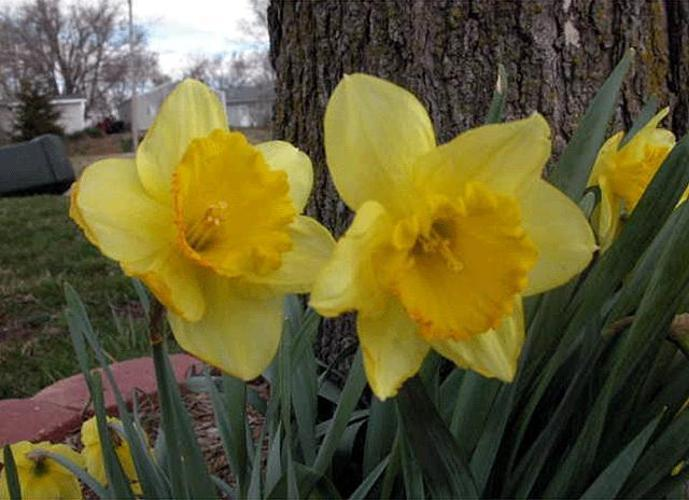
\includegraphics[width=0.165\textwidth]{cc_demo/flower001_base.png}&
    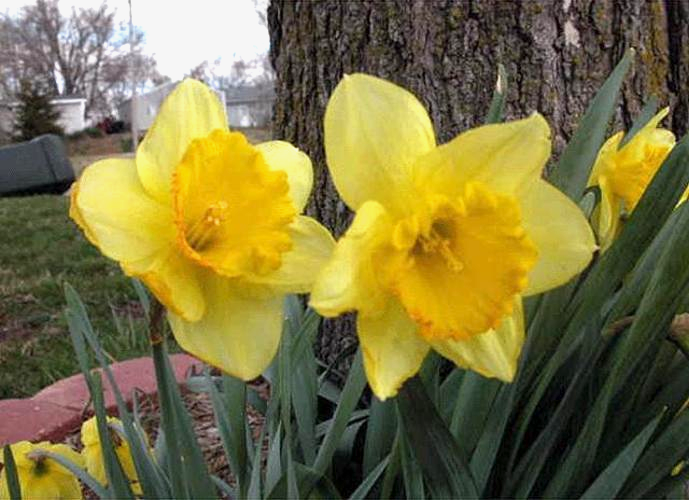
\includegraphics[width=0.165\textwidth]{cc_demo/flower001_whitePatch.png}&
    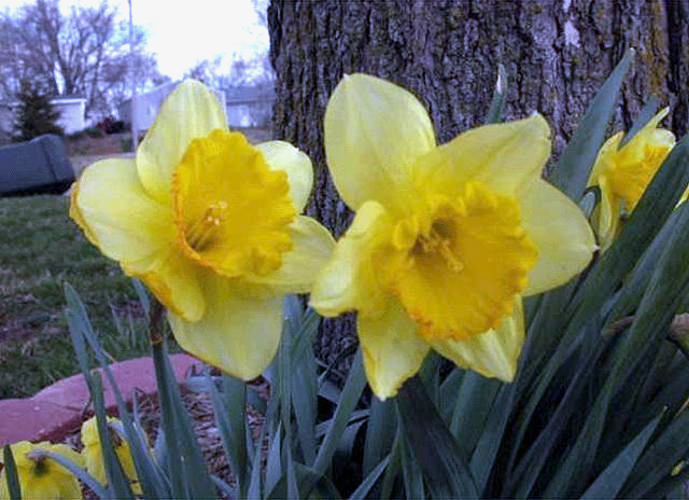
\includegraphics[width=0.165\textwidth]{cc_demo/flower001_greyWorld.png}&
    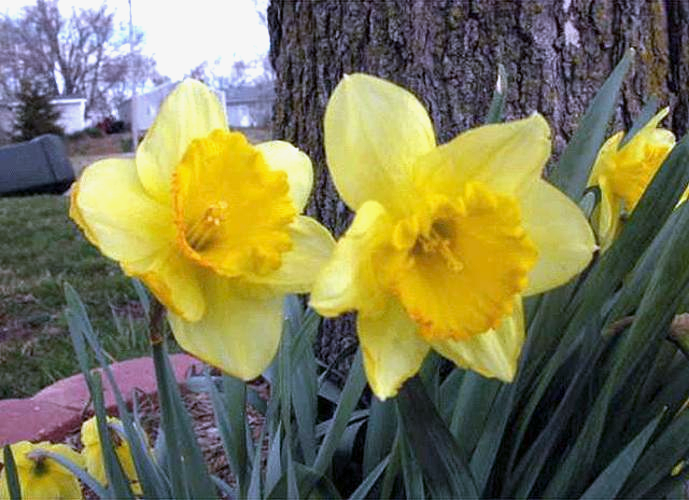
\includegraphics[width=0.165\textwidth]{cc_demo/flower001_grayEdge.png}&
    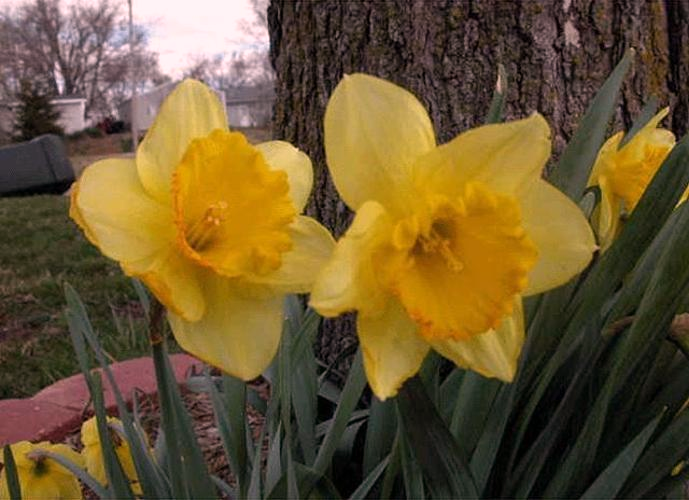
\includegraphics[width=0.165\textwidth]{cc_demo/flower001_fc4.png}\\
    (a)&(b)&(c)&(d)&(e)\\
    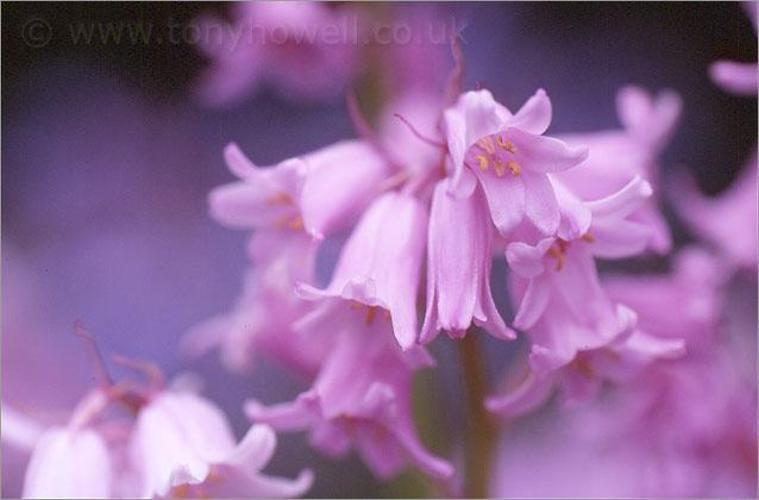
\includegraphics[width=0.165\textwidth]{cc_demo/flower268_base.png}&
    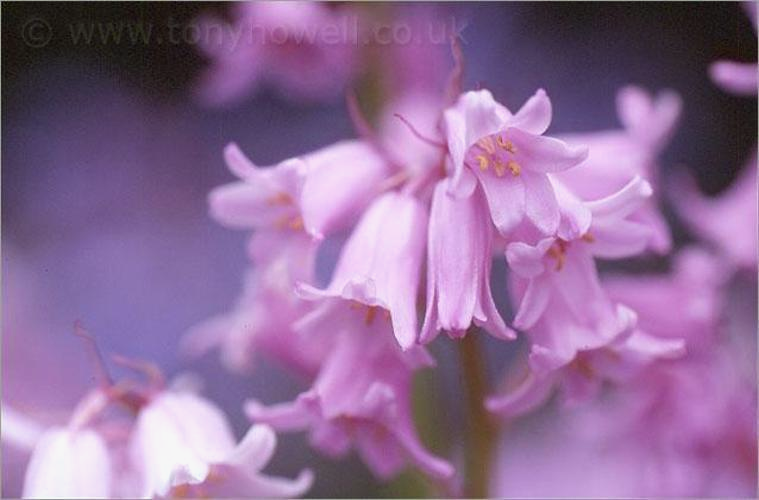
\includegraphics[width=0.165\textwidth]{cc_demo/flower268_whitePatch.png}&
    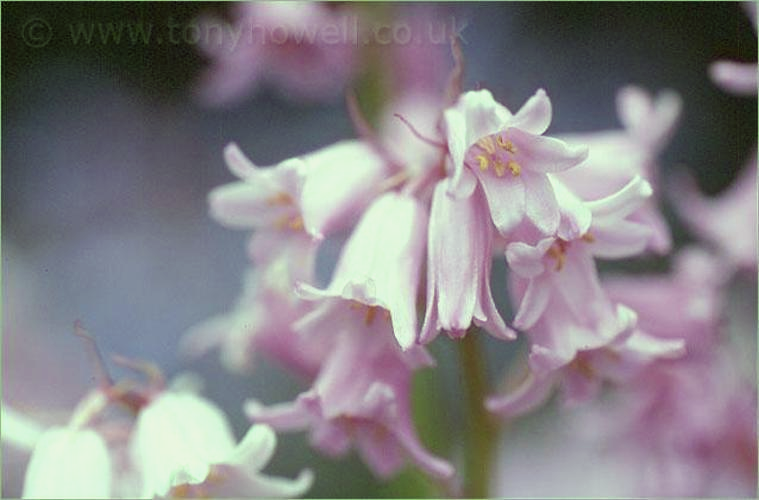
\includegraphics[width=0.165\textwidth]{cc_demo/flower268_greyWorld.png}&
    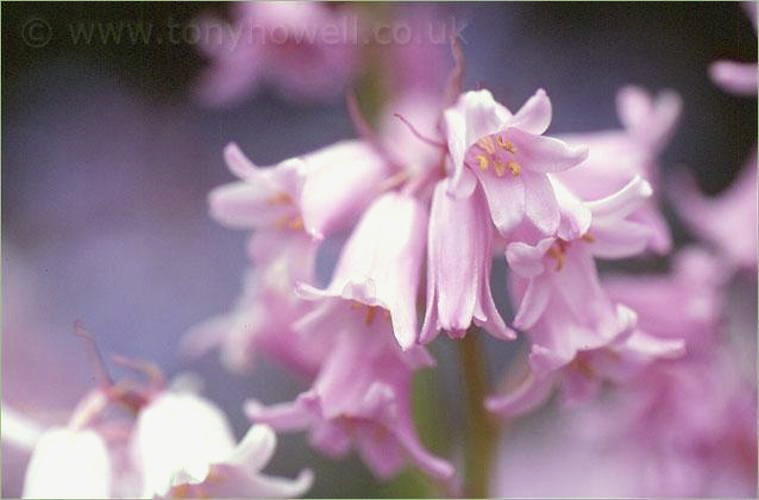
\includegraphics[width=0.165\textwidth]{cc_demo/flower268_grayEdge.png}&
    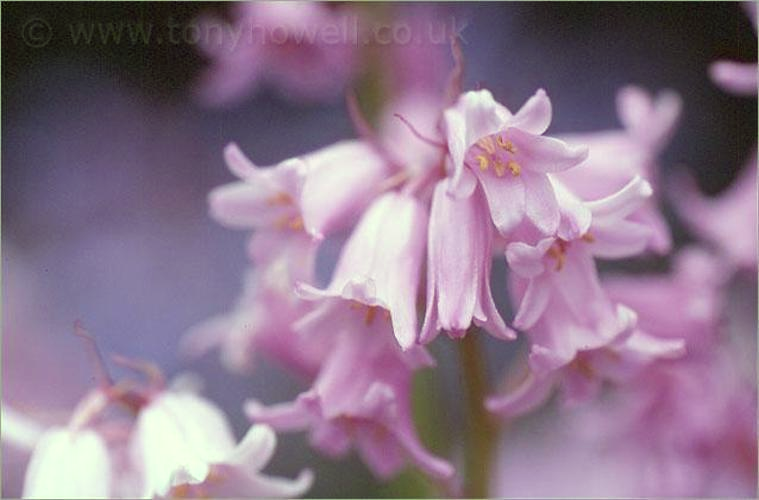
\includegraphics[width=0.165\textwidth]{cc_demo/flower268_fc4.png}\\
    (f)&(g)&(h)&(i)&(j)
    \end{tabular}
    \caption{A comparison of color constancy algorithms: (a) and (f): Original image.
        (b) and (g): White Patch. (c) and (h): Grey-World. 
        (d) and (i): Grey-Edge. (e) and (j): FC\textsuperscript{4}}
    \label{fig:cc_comparison}
\end{figure}

In order to have a wider spread of examined methods, we both make use of state-of-the art 
learning based methods (in this case represented by FC\textsuperscript{4}\cite{hu2017fc}), as well as classical simpler methods 
like White-Patch, Grey-World \cite{EbnerConstancy} and Grey-Edge \cite{van2005color}.
A comparison of these can be found in \ref{fig:cc_comparison}.

\subsubsection{Statistical Methods}

In the grey world algorithm, the assumption is made that the average reflectance of the scene should
be a shade of grey. We can therefore infer that any deviation of the average color from this grey tone stems from
the illumination in the scene. By simply dividing this out, we receive a color-corrected image.

White-Patch is a close relative of this method, where instead we assume that the brightest spot in the image (for each channel)
is representative of the overall light color.

In the grey-edge hypothesis we instead assume that the average image gradient can be used as an indication of the light color.

All of these algorithms were reimplemented by us. Notably, based on the recommendation made by Ebner \cite{EbnerConstancy},
after color adjustment we rescale all results such that the top 5\% of values (across all channels) will be clipped to
the maximum intensity of 1.

\subsection{Classification models}

Two classification models were used for the classification stage of the pipeline: Pre-trained VGG16 and our own implemented network. % FUNY-NET

\subsubsection{VGG16}
We utilized a pre-trained VGG16 convolutional neural network architecture to classify a raw 17 category image dataset. 
The model was obtained from an online source and trained on our dataset. During training, the model achieved a training accuracy of 0.8446691036224365 and a test accuracy of 0.7867646813392639. 
The training accuracy score indicates the model's performance on the training data, while the test accuracy score represents the model's generalization ability on unseen data. 
The difference between the training and test accuracy scores suggests that the model might be overfitting to the training data. Therefore, further investigation may be needed to improve the model's performance on unseen data.
Overall, the achieved accuracy scores demonstrate the potential of the VGG16 model for classifying the given image dataset. 

\subsubsection{Our Implemented Classifier}
The initial version of our network is composed of a convolution layer, followed by max pooling, flatten, and a dense layer, finishing with a softmax activation. 
The goal of the initial version is to verify that the dataset was preprocessed in a way that allows fitting and evaluating the model, and to later tune it.
For this, the 17 flowers dataset was split into training and validation sets (with the test set split to be implemented later) in a 80/20 ratio and used to fit the model.

Once the fitting was successful and it was verified that the dataset splits work, we implemented the basis for model tuning using the Keras Tuner \cite{omalley2019kerastuner}.
Number of filters and the kernel size in the convolution layer were the focus of the tuning trial, with values varying from 32 to 512 with steps of 32 for the number of filters, and kernel sizes of 3 and 5.
Number of trials was set to 3, max pooling kernel size of 2x2, Adam optimizer, and Sparse Categorical Crossentropy for the loss function. Trial results are as follows:

\begin{tabular}{c|c|c}
    Filters&Kernel size&Score\\
    \hline
    \hline
    224&3x3&0.5515\\
    \hline
    320&5x5&0.5000\\
    \hline
    32&5x5&0.4890
\end{tabular}

This verifies that we can easily tune our network as we develop it further. It's clear that the score is low and the model can be further improved with additional layers.
Furthermore, it was noted that the model quickly overfits past epoch number $5$ with an accuracy of around $0.99$ but validation score of approximately $0.5$.
The use of, e.g., dropout layers and other techniques could help avoid overfitting.

Next steps include adding more layers to the model, implementing features to avoid overfitting (i.e., dropout), experimenting with a depthwise and depthwise-separable convolution approach, and applying FUNY-NET to the datasets preprocessed by the CC models.

\pgfplotstabletypeset[
    col sep=comma,
    columns={Algorithm, Average Train Time, Average Test Time, 
        Average Training Loss, Average Validation Loss, Average Test Accuracy},
    column type = l,
    columns/Algorithm/.style={string type, column name=},
    columns/Average Train Time/.style = {column name ={Training (s)}},
    columns/Average Test Time/.style = {column name ={Testing (s)}},
    columns/Average Training Loss/.style = {column name ={Train Loss}},
    columns/Average Validation Loss/.style = {column name ={Val Loss}},
    columns/Average Test Accuracy/.style = {column name ={Test Acc}},
    every head row/.style = {before row=\hline, after row=\hline},
    every last row/.style = {after row=\hline},
    every column/.style = {column type/.add={|}{}},
    every last column/.style = {column type/.add={}{|}}
]{data/ours_17_flowers_summary.csv}

\begin{figure}
    \centering
    \begin{tabular}{cc}
        \begin{tikzpicture}
            \begin{axis}[
                title = Training Time,
                ylabel = time/s,
                ybar,
                xtick=data,
                xticklabels from table = {data/ours_17_flowers_summary.csv}{Algorithm},
                x tick label style = {rotate=45, anchor=east},
                error bars/y dir=both,
                error bars/y explicit,
                error bars/error bar style={black},
                ymin=0,
                width=0.49\textwidth,
                bar width=6,
            ]
                \addplot+[
                    title = Our Model,
                    draw=black,
                    fill=ourorange,
                ] table[
                    col sep=comma,
                    x expr=\coordindex,
                    y=Average Train Time,
                    y error=Stdev Train Time
                ] {data/ours_17_flowers_summary.csv};
                \addplot+[
                    title = Our Model,
                    draw=black,
                    fill=ourblue
                ] table[
                    col sep=comma,
                    x expr=\coordindex,
                    y=Average Train Time,
                    y error=Stdev Train Time
                ] {data/ours_17_flowers_summary.csv};
            \end{axis}
        \end{tikzpicture}&
        \begin{tikzpicture}
            \begin{axis}[
                title = Testing Time,
                xtick=data,
                xticklabels from table = {data/ours_17_flowers_summary.csv}{Algorithm},
                x tick label style = {rotate=45, anchor=east},
                error bars/y dir=both,
                error bars/y explicit,
                error bars/error bar style={black},
                no markers,
                ymin=0,
                width=0.49\textwidth,
            ]
                \addplot+[
                    title = Our Model,
                    ybar,
                    draw=black,
                    fill=ourblue
                ] table[
                    col sep=comma,
                    x expr=\coordindex,
                    y=Average Test Time,
                    y error=Stdev Test Time
                ] {data/ours_17_flowers_summary.csv};
            \end{axis}
        \end{tikzpicture}
    \end{tabular}

    \begin{tikzpicture}
        \begin{axis}[
            title = Validation Loss over Time,
            mark repeat=4,
            xlabel = Epoch,
            ylabel = Loss,
        ]
            \addplot+[
                sharp plot,
            ] table[
                x = Epoch,
                y = Base,
            ] {data/validation_loss_17_flowers.csv};
            \addlegendentry{Base}
            \addplot+[
                sharp plot,
            ] table[
                x = Epoch,
                y = BatchNorm,
            ] {data/validation_loss_17_flowers.csv};
            \addlegendentry{Batch Norm}
            \addplot+[
                sharp plot,
            ] table[
                x = Epoch,
                y = FC4,
            ] {data/validation_loss_17_flowers.csv};
            \addlegendentry{FC\textsuperscript{4}}
            \addplot+[
                sharp plot,
            ] table[
                x = Epoch,
                y = WhitePatch,
            ] {data/validation_loss_17_flowers.csv};
            \addlegendentry{White Patch}
            \addplot+[
                sharp plot,
            ] table[
                x = Epoch,
                y = GreyEdge,
            ] {data/validation_loss_17_flowers.csv};
            \addlegendentry{Grey Edge}
            \addplot+[
                sharp plot,
            ] table[
                x = Epoch,
                y = GreyWorld,
            ] {data/validation_loss_17_flowers.csv};
            \addlegendentry{Grey World}
        \end{axis}
    \end{tikzpicture}

    \begin{tikzpicture}
        \begin{axis}[
            title = Validation Accuracy over Time,
            mark repeat=4,
            xlabel = Epoch,
            ylabel = Accuracy,
            legend pos=south east,
        ]
            \addplot+[
                sharp plot,
            ] table[
                x = Epoch,
                y = Base,
            ] {data/validation_accuracy_17_flowers.csv};
            \addlegendentry{Base}
            \addplot+[
                sharp plot,
            ] table[
                x = Epoch,
                y = BatchNorm,
            ] {data/validation_accuracy_17_flowers.csv};
            \addlegendentry{Batch Norm}
            \addplot+[
                sharp plot,
            ] table[
                x = Epoch,
                y = FC4,
            ] {data/validation_accuracy_17_flowers.csv};
            \addlegendentry{FC\textsuperscript{4}}
            \addplot+[
                sharp plot,
            ] table[
                x = Epoch,
                y = WhitePatch,
            ] {data/validation_accuracy_17_flowers.csv};
            \addlegendentry{White Patch}
            \addplot+[
                sharp plot,
            ] table[
                x = Epoch,
                y = GreyEdge,
            ] {data/validation_accuracy_17_flowers.csv};
            \addlegendentry{Grey Edge}
            \addplot+[
                sharp plot,
            ] table[
                x = Epoch,
                y = GreyWorld,
            ] {data/validation_accuracy_17_flowers.csv};
            \addlegendentry{Grey World}
        \end{axis}
    \end{tikzpicture}
    \caption{A bar chart to test with.}
    \label{fig:testbar}
\end{figure}